
%% bare_conf.tex
%% V1.4
%% 2012/12/27
%% by Michael Shell
%% See:
%% http://www.michaelshell.org/
%% for current contact information.
%%
%% This is a skeleton file demonstrating the use of IEEEtran.cls
%% (requires IEEEtran.cls version 1.8 or later) with an IEEE conference paper.
%%
%% Support sites:
%% http://www.michaelshell.org/tex/ieeetran/
%% http://www.ctan.org/tex-archive/macros/latex/contrib/IEEEtran/
%% and
%% http://www.ieee.org/

%%*************************************************************************
%% Legal Notice:
%% This code is offered as-is without any warranty either expressed or
%% implied; without even the implied warranty of MERCHANTABILITY or
%% FITNESS FOR A PARTICULAR PURPOSE! 
%% User assumes all risk.
%% In no event shall IEEE or any contributor to this code be liable for
%% any damages or losses, including, but not limited to, incidental,
%% consequential, or any other damages, resulting from the use or misuse
%% of any information contained here.
%%
%% All comments are the opinions of their respective authors and are not
%% necessarily endorsed by the IEEE.
%%
%% This work is distributed under the LaTeX Project Public License (LPPL)
%% ( http://www.latex-project.org/ ) version 1.3, and may be freely used,
%% distributed and modified. A copy of the LPPL, version 1.3, is included
%% in the base LaTeX documentation of all distributions of LaTeX released
%% 2003/12/01 or later.
%% Retain all contribution notices and credits.
%% ** Modified files should be clearly indicated as such, including  **
%% ** renaming them and changing author support contact information. **
%%
%% File list of work: IEEEtran.cls, IEEEtran_HOWTO.pdf, bare_adv.tex,
%%                    bare_conf.tex, bare_jrnl.tex, bare_jrnl_compsoc.tex,
%%                    bare_jrnl_transmag.tex
%%*************************************************************************

% *** Authors should verify (and, if needed, correct) their LaTeX system  ***
% *** with the testflow diagnostic prior to trusting their LaTeX platform ***
% *** with production work. IEEE's font choices can trigger bugs that do  ***
% *** not appear when using other class files.                            ***
% The testflow support page is at:
% http://www.michaelshell.org/tex/testflow/



% Note that the a4paper option is mainly intended so that authors in
% countries using A4 can easily print to A4 and see how their papers will
% look in print - the typesetting of the document will not typically be
% affected with changes in paper size (but the bottom and side margins will).
% Use the testflow package mentioned above to verify correct handling of
% both paper sizes by the user's LaTeX system.
%
% Also note that the "draftcls" or "draftclsnofoot", not "draft", option
% should be used if it is desired that the figures are to be displayed in
% draft mode.
%
\documentclass[conference]{IEEEtran}
% Add the compsoc option for Computer Society conferences.
%
% If IEEEtran.cls has not been installed into the LaTeX system files,
% manually specify the path to it like:
% \documentclass[conference]{../sty/IEEEtran}


\usepackage{listings}


% Some very useful LaTeX packages include:
% (uncomment the ones you want to load)


% *** MISC UTILITY PACKAGES ***
%
%\usepackage{ifpdf}
% Heiko Oberdiek's ifpdf.sty is very useful if you need conditional
% compilation based on whether the output is pdf or dvi.
% usage:
% \ifpdf
%   % pdf code
% \else
%   % dvi code
% \fi
% The latest version of ifpdf.sty can be obtained from:
% http://www.ctan.org/tex-archive/macros/latex/contrib/oberdiek/
% Also, note that IEEEtran.cls V1.7 and later provides a builtin
% \ifCLASSINFOpdf conditional that works the same way.
% When switching from latex to pdflatex and vice-versa, the compiler may
% have to be run twice to clear warning/error messages.






% *** CITATION PACKAGES ***
%
%\usepackage{cite}
% cite.sty was written by Donald Arseneau
% V1.6 and later of IEEEtran pre-defines the format of the cite.sty package
% \cite{} output to follow that of IEEE. Loading the cite package will
% result in citation numbers being automatically sorted and properly
% "compressed/ranged". e.g., [1], [9], [2], [7], [5], [6] without using
% cite.sty will become [1], [2], [5]--[7], [9] using cite.sty. cite.sty's
% \cite will automatically add leading space, if needed. Use cite.sty's
% noadjust option (cite.sty V3.8 and later) if you want to turn this off
% such as if a citation ever needs to be enclosed in parenthesis.
% cite.sty is already installed on most LaTeX systems. Be sure and use
% version 4.0 (2003-05-27) and later if using hyperref.sty. cite.sty does
% not currently provide for hyperlinked citations.
% The latest version can be obtained at:
% http://www.ctan.org/tex-archive/macros/latex/contrib/cite/
% The documentation is contained in the cite.sty file itself.






% *** GRAPHICS RELATED PACKAGES ***
%
\ifCLASSINFOpdf
\usepackage{tikz}
\usetikzlibrary{chains}
\usetikzlibrary{shapes.geometric, arrows}
\usetikzlibrary{trees}
  % \usepackage[pdftex]{graphicx}
  % declare the path(s) where your graphic files are
  % \graphicspath{{../pdf/}{../jpeg/}}
  % and their extensions so you won't have to specify these with
  % every instance of \includegraphics
  % \DeclareGraphicsExtensions{.pdf,.jpeg,.png}
\else
  % or other class option (dvipsone, dvipdf, if not using dvips). graphicx
  % will default to the driver specified in the system graphics.cfg if no
  % driver is specified.
  % \usepackage[dvips]{graphicx}
  % declare the path(s) where your graphic files are
  % \graphicspath{{../eps/}}
  % and their extensions so you won't have to specify these with
  % every instance of \includegraphics
  % \DeclareGraphicsExtensions{.eps}
\fi
% graphicx was written by David Carlisle and Sebastian Rahtz. It is
% required if you want graphics, photos, etc. graphicx.sty is already
% installed on most LaTeX systems. The latest version and documentation
% can be obtained at: 
% http://www.ctan.org/tex-archive/macros/latex/required/graphics/
% Another good source of documentation is "Using Imported Graphics in
% LaTeX2e" by Keith Reckdahl which can be found at:
% http://www.ctan.org/tex-archive/info/epslatex/
%
% latex, and pdflatex in dvi mode, support graphics in encapsulated
% postscript (.eps) format. pdflatex in pdf mode supports graphics
% in .pdf, .jpeg, .png and .mps (metapost) formats. Users should ensure
% that all non-photo figures use a vector format (.eps, .pdf, .mps) and
% not a bitmapped formats (.jpeg, .png). IEEE frowns on bitmapped formats
% which can result in "jaggedy"/blurry rendering of lines and letters as
% well as large increases in file sizes.
%
% You can find documentation about the pdfTeX application at:
% http://www.tug.org/applications/pdftex





% *** MATH PACKAGES ***
%
%\usepackage[cmex10]{amsmath}
% A popular package from the American Mathematical Society that provides
% many useful and powerful commands for dealing with mathematics. If using
% it, be sure to load this package with the cmex10 option to ensure that
% only type 1 fonts will utilized at all point sizes. Without this option,
% it is possible that some math symbols, particularly those within
% footnotes, will be rendered in bitmap form which will result in a
% document that can not be IEEE Xplore compliant!
%
% Also, note that the amsmath package sets \interdisplaylinepenalty to 10000
% thus preventing page breaks from occurring within multiline equations. Use:
%\interdisplaylinepenalty=2500
% after loading amsmath to restore such page breaks as IEEEtran.cls normally
% does. amsmath.sty is already installed on most LaTeX systems. The latest
% version and documentation can be obtained at:
% http://www.ctan.org/tex-archive/macros/latex/required/amslatex/math/





% *** SPECIALIZED LIST PACKAGES ***
%
%\usepackage{algorithmic}
% algorithmic.sty was written by Peter Williams and Rogerio Brito.
% This package provides an algorithmic environment fo describing algorithms.
% You can use the algorithmic environment in-text or within a figure
% environment to provide for a floating algorithm. Do NOT use the algorithm
% floating environment provided by algorithm.sty (by the same authors) or
% algorithm2e.sty (by Christophe Fiorio) as IEEE does not use dedicated
% algorithm float types and packages that provide these will not provide
% correct IEEE style captions. The latest version and documentation of
% algorithmic.sty can be obtained at:
% http://www.ctan.org/tex-archive/macros/latex/contrib/algorithms/
% There is also a support site at:
% http://algorithms.berlios.de/index.html
% Also of interest may be the (relatively newer and more customizable)
% algorithmicx.sty package by Szasz Janos:
% http://www.ctan.org/tex-archive/macros/latex/contrib/algorithmicx/




% *** ALIGNMENT PACKAGES ***
%
%\usepackage{array}
% Frank Mittelbach's and David Carlisle's array.sty patches and improves
% the standard LaTeX2e array and tabular environments to provide better
% appearance and additional user controls. As the default LaTeX2e table
% generation code is lacking to the point of almost being broken with
% respect to the quality of the end results, all users are strongly
% advised to use an enhanced (at the very least that provided by array.sty)
% set of table tools. array.sty is already installed on most systems. The
% latest version and documentation can be obtained at:
% http://www.ctan.org/tex-archive/macros/latex/required/tools/


% IEEEtran contains the IEEEeqnarray family of commands that can be used to
% generate multiline equations as well as matrices, tables, etc., of high
% quality.




% *** SUBFIGURE PACKAGES ***
%\ifCLASSOPTIONcompsoc
%  \usepackage[caption=false,font=normalsize,labelfont=sf,textfont=sf]{subfig}
%\else
%  \usepackage[caption=false,font=footnotesize]{subfig}
%\fi
% subfig.sty, written by Steven Douglas Cochran, is the modern replacement
% for subfigure.sty, the latter of which is no longer maintained and is
% incompatible with some LaTeX packages including fixltx2e. However,
% subfig.sty requires and automatically loads Axel Sommerfeldt's caption.sty
% which will override IEEEtran.cls' handling of captions and this will result
% in non-IEEE style figure/table captions. To prevent this problem, be sure
% and invoke subfig.sty's "caption=false" package option (available since
% subfig.sty version 1.3, 2005/06/28) as this is will preserve IEEEtran.cls
% handling of captions.
% Note that the Computer Society format requires a larger sans serif font
% than the serif footnote size font used in traditional IEEE formatting
% and thus the need to invoke different subfig.sty package options depending
% on whether compsoc mode has been enabled.
%
% The latest version and documentation of subfig.sty can be obtained at:
% http://www.ctan.org/tex-archive/macros/latex/contrib/subfig/




% *** FLOAT PACKAGES ***
%
%\usepackage{fixltx2e}
% fixltx2e, the successor to the earlier fix2col.sty, was written by
% Frank Mittelbach and David Carlisle. This package corrects a few problems
% in the LaTeX2e kernel, the most notable of which is that in current
% LaTeX2e releases, the ordering of single and double column floats is not
% guaranteed to be preserved. Thus, an unpatched LaTeX2e can allow a
% single column figure to be placed prior to an earlier double column
% figure. The latest version and documentation can be found at:
% http://www.ctan.org/tex-archive/macros/latex/base/


%\usepackage{stfloats}
% stfloats.sty was written by Sigitas Tolusis. This package gives LaTeX2e
% the ability to do double column floats at the bottom of the page as well
% as the top. (e.g., "\begin{figure*}[!b]" is not normally possible in
% LaTeX2e). It also provides a command:
%\fnbelowfloat
% to enable the placement of footnotes below bottom floats (the standard
% LaTeX2e kernel puts them above bottom floats). This is an invasive package
% which rewrites many portions of the LaTeX2e float routines. It may not work
% with other packages that modify the LaTeX2e float routines. The latest
% version and documentation can be obtained at:
% http://www.ctan.org/tex-archive/macros/latex/contrib/sttools/
% Do not use the stfloats baselinefloat ability as IEEE does not allow
% \baselineskip to stretch. Authors submitting work to the IEEE should note
% that IEEE rarely uses double column equations and that authors should try
% to avoid such use. Do not be tempted to use the cuted.sty or midfloat.sty
% packages (also by Sigitas Tolusis) as IEEE does not format its papers in
% such ways.
% Do not attempt to use stfloats with fixltx2e as they are incompatible.
% Instead, use Morten Hogholm'a dblfloatfix which combines the features
% of both fixltx2e and stfloats:
%
% \usepackage{dblfloatfix}
% The latest version can be found at:
% http://www.ctan.org/tex-archive/macros/latex/contrib/dblfloatfix/




% *** PDF, URL AND HYPERLINK PACKAGES ***
%
%\usepackage{url}
% url.sty was written by Donald Arseneau. It provides better support for
% handling and breaking URLs. url.sty is already installed on most LaTeX
% systems. The latest version and documentation can be obtained at:
% http://www.ctan.org/tex-archive/macros/latex/contrib/url/
% Basically, \url{my_url_here}.




% *** Do not adjust lengths that control margins, column widths, etc. ***
% *** Do not use packages that alter fonts (such as pslatex).         ***
% There should be no need to do such things with IEEEtran.cls V1.6 and later.
% (Unless specifically asked to do so by the journal or conference you plan
% to submit to, of course. )


% correct bad hyphenation here
\hyphenation{op-tical net-works semi-conduc-tor}


\begin{document}
%
% paper title
% can use linebreaks \\ within to get better formatting as desired
% Do not put math or special symbols in the title.
\title{OS II Project Report: Rust Kernel}


% author names and affiliations
% use a multiple column layout for up to three different
% affiliations
\author{\IEEEauthorblockN{Jianzhong Liu	}
\IEEEauthorblockA{School of Information Science and Technology\\
ShanghaiTech University\\
Shanghai, China 201210\\
Email: liujzh@shanghaitech.edu.cn}
}

% conference papers do not typically use \thanks and this command
% is locked out in conference mode. If really needed, such as for
% the acknowledgment of grants, issue a \IEEEoverridecommandlockouts
% after \documentclass

% for over three affiliations, or if they all won't fit within the width
% of the page, use this alternative format:
% 
%\author{\IEEEauthorblockN{Michael Shell\IEEEauthorrefmark{1},
%Homer Simpson\IEEEauthorrefmark{2},
%James Kirk\IEEEauthorrefmark{3}, 
%Montgomery Scott\IEEEauthorrefmark{3} and
%Eldon Tyrell\IEEEauthorrefmark{4}}
%\IEEEauthorblockA{\IEEEauthorrefmark{1}School of Electrical and Computer Engineering\\
%Georgia Institute of Technology,
%Atlanta, Georgia 30332--0250\\ Email: see http://www.michaelshell.org/contact.html}
%\IEEEauthorblockA{\IEEEauthorrefmark{2}Twentieth Century Fox, Springfield, USA\\
%Email: homer@thesimpsons.com}
%\IEEEauthorblockA{\IEEEauthorrefmark{3}Starfleet Academy, San Francisco, California 96678-2391\\
%Telephone: (800) 555--1212, Fax: (888) 555--1212}
%\IEEEauthorblockA{\IEEEauthorrefmark{4}Tyrell Inc., 123 Replicant Street, Los Angeles, California 90210--4321}}




% use for special paper notices
%\IEEEspecialpapernotice{(Invited Paper)}




% make the title area
\maketitle

% As a general rule, do not put math, special symbols or citations
% in the abstract
\begin{abstract}
This report will mainly discuss the results and findings on implementing an operating system kernel in the programming language Rust. We will first cover the overall structure of the system. Systems programming in Rust yields many benefits over programming in C or other traditional languages, thus we will also discuss the advantages and pitfalls of using Rust as a systems programming language.
\end{abstract}

% no keywords




% For peer review papers, you can put extra information on the cover
% page as needed:
% \ifCLASSOPTIONpeerreview
% \begin{center} \bfseries EDICS Category: 3-BBND \end{center}
% \fi
%
% For peerreview papers, this IEEEtran command inserts a page break and
% creates the second title. It will be ignored for other modes.
\IEEEpeerreviewmaketitle



\section{Introduction}
% no \IEEEPARstart

The Rust programming language as a systems programming language presents many opportunities to improve upon the classical mindset of bare bones programming, especially in kernel programming. As an operating systems course project, programming a kernel in Rust offers experience in bare bones programming, operating system kernel structure implementation and Rust bare metal programming.

Given the significant benefits, I chose to implement a simple kernel in Rust to understand the internals of an operating system better while utilizing a modern programming language.

\section{Kernel Outline}

The kernel implemented is targeted for the x86-64 architecture that is prevalent in modern PCs. It is based on a monolithic kernel philosophy, which integrates main functionalities in the kernel space exposing a comprehensive system call interface to user applications. The tasks to support and an overall structure is shown below.

\subsection{Kernel Tasks}

\subsubsection{Paging Management}

Modern ISAs use paging to manage memory address translation while segmentation is mostly ignored. The kernel has to keep in track of pages allocated and the mapping between virtual pages and physical frames.

\subsubsection{Interrupt Handling}

Current ISAs are interrupt driven, thus the kernel will need to handle interrupts to manage system events, both external and internal. Furthermore, the kernel will need to return from interrupts and present a transparent interrupt model to the user program.

\subsubsection{I/O Communication Handling and Abstraction}

The kernel would also need to handle I/O communications and abstractions, so that user programs would have a unified programming model to handle I/O usage.

\subsubsection{Network Stack Management}

The kernel would have to maintain a kernel space network stack so that the operating system can provide networking functionality to the user programs.

\subsubsection{File System Abstraction}

A good file system abstraction would also be needed to be compatible with various file system formats while exposing a unified virtual file system to the user process.

\subsubsection{Task Spawning, Management and Scheduling}

The kernel will also have to support loading user space executables, maintaining running programs and schedule processes to share CPU time slices.

\subsubsection{Permission Handling}

The kernel will have to maintain a permission system to handle system-wide activities so that different users will have different levels of permissions.

\subsection{Kernel Architecture}

The main architecture for the kernel is shown in the graph below:

\begin{center}
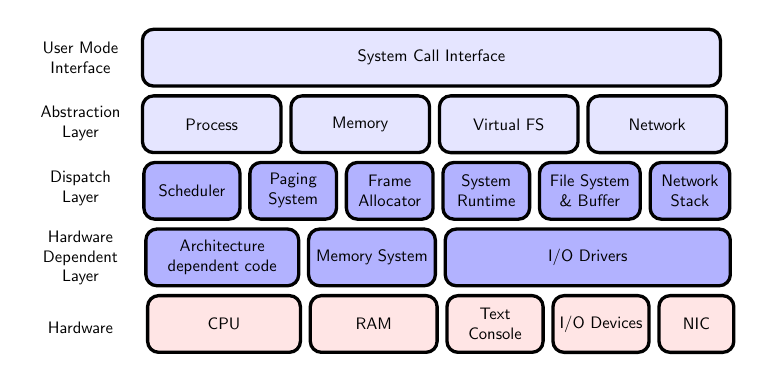
\begin{tikzpicture}[
scale=0.75,
start chain=1 going below, 
start chain=2 going right,
node distance=1mm,
desc/.style={
	scale=0.75,
	on chain=2,
	rectangle,
	rounded corners,
	draw=black, 
	very thick,
	text centered,
	text width=12cm,
	minimum height=12mm,
	fill=blue!30
},
it/.style={
	fill=blue!10
},
hw/.style={
	fill=red!10
},
level/.style={
	scale=0.75,
	on chain=1,
	minimum height=12mm,
	text width=2cm,
	text centered
},
every node/.style={font=\sffamily,scale=0.8}
]

% Levels
\node [level] (Level 4) {User Mode Interface};
\node [level] (Level 3) {Abstraction Layer};
\node [level] (Level 2) {Dispatch Layer};
\node [level] (Level 1) {Hardware Dependent Layer};
\node [level] (Level 0) {Hardware};

% Descriptions
\chainin (Level 4); % Start right of Level 5
\node [desc, it] (Syscall) {System Call Interface};
\node [desc, it, continue chain=going below, text width= 2.7cm, xshift=-4.65cm] (Proc) {Process};
\node [desc, it, continue chain=going right, text width= 2.7cm] (Proc) {Memory};
\node [desc, it, text width= 2.7cm] (vfs) {Virtual FS};
\node [desc, it, text width= 2.7cm] (net) {Network};
\node [desc, continue chain=going below, text width= 1.8cm, xshift=-9.85cm] (Sched) {Scheduler};
\node [desc, continue chain=going right, text width= 1.6cm] (pgsys) {Paging System};
\node [desc,  text width= 1.6cm] (frmalloc) {Frame Allocator};
\node [desc,  text width= 1.6cm] (sysrt) {System Runtime};
\node [desc,  text width= 1.9cm] (fs) {File System \& Buffer};
\node [desc, text width=1.45cm] (ns) {Network Stack};
\node [desc, continue chain=going below, text width= 3cm, xshift=-9.9cm] (arch) {Architecture dependent code};
\node [desc, continue chain=going right, text width=2.45cm] (mmu) {Memory System};
\node [desc,  text width= 5.8cm] (iodrivers) {I/O Drivers};
\node [desc, hw, continue chain=going below, text width=3cm, xshift=-7.7cm] (cpu) {CPU};
\node [desc, hw, continue chain=going right, text width=2.45cm] (mem) {RAM};
\node [desc, hw, text width= 1.8cm] (con) {Text Console};
\node [desc, hw, text width= 1.8cm] (dev) {I/O Devices};
\node [desc, hw, text width= 1.35cm] (nic) {NIC};

\end{tikzpicture}
\end{center}

\subsubsection{User Mode Interface}

This level exposes a comprehensive set of system calls to the user program in order to utilize kernel functionalities.

\subsubsection{Abstraction Layer}

This layer abstracts the specific function call functionality into four separate categories:

\begin{itemize}
		\item Process: Functions related with scheduling and managing processes
	\item Memory: Functions related with memory management
	\item Virtual FS: Functions providing access to an abstracted view of the system's resources represented as items in a virtual file system
	\item Network: Functions that provide socket and network functionality
\end{itemize}

\subsubsection{Dispatch Layer}

This layer presents different subsystems to handle specific functionalities. They maintain data structures representing the system state and dispatch specific instructions to the specific hardware specific implementation.

\subsubsection{Hardware Dependent Layer}

This layer is hardware dependent, thus exposing a unified function call across architectures that uses different implementations for different ISAs.

\section{Implementation Details}

Here we present the implementation details related to this kernel. Since it is still a work in progress, some details will be specified to be TODO.

\subsection{Kernel Boot and Setup}

The kernel boot and setup process is intensely architecture dependent. Thus the x86-64 architecture (or x64, amd64) will be used as an example to demonstrate the tasks involved upon system boot.

\subsubsection{BIOS to bootloader}

The system will perform POST and after identifying the boot drive, will load the MBR into memory. Then the bootloader will load itself into memory, setup segmentation, paging, GDT (Global Descriptor Table) and transition to protected mode, which is the 32-bit operation mode for this architecture. From there it hands control over to the kernel.

The kernel we implemented complies with the Multiboot 2 specifications, thus we are able to load the kernel using any Multiboot 2 bootloader. GRUB (GRand Unified Bootloader) is the bootloader of our choice.

\subsubsection{CPU Checks}

The kernel will perform checks verifying that the CPU supports long mode so that we may switch to 64-bit mode successfully. If the CPU is not 64-bit compliant, the kernel boot process will halt.

\subsubsection{Setup Identity Mapped Page Tables}

Since the 64-bit architecture uses paging for all memory accessing, we would need to load an identity mapped page table so we wouldn't trap into a page fault once we made the switch.

For this purpose, we allocated multiple 4K pages statically and set their contents to be an identity mapped page table. For convenience purposes we only used three levels of page tables, using huge tables to map the first 1GiB of memory.

\subsubsection{Setup GDT}

For backwards compatibility we would also need a basic GDT (Global Descriptor Table) to ensure that memory is accessible using segmentation, though segment limits are mostly ignored under 64-bit mode. The GDT looks like this:

\begin{verbatim}
    section .rodata
gdt64:
    dq 0x0
.code: equ $ - gdt64
    dq (1<<43) | (1<<44) | (1<<47) | (1<<53)
.pointer:
    dw $ - gdt64 - 1
    dq gdt64
\end{verbatim}

This allocates one large code segment and makes the processor happy.

\subsubsection{Load Rudimentary IDT}

We would also need to load a very basic IDT so in the event of a processor exception happening before loading useful ISRs (Interrupt Service Routine) we would be notified and the processor would not trap into a triple fault which would result in a system reset.

The basic ISR for each interrupt is basically the same. We print out error messages and halt, which is enough for our purposes. Meaningful ISRs will be loaded after we make the switch to 64-bit mode.

\subsubsection{Long Jump to 64-bit Mode}

After setting up the page tables, GDT and IDT, we have already switched to long mode. We just need a long jump to clear out the segment registers and switch to 64-bit mode. Therefore we use 
\begin{verbatim}
jmp gdt64.code:long_start
\end{verbatim}
to make the switch to 64-bit mode.

\subsubsection{Jump to Rust Code}

To hand control over to the Rust code, we would need to specify the ABI for the Rust code for the function call to be successful. Therefore we define the Rust main function to be 

\begin{verbatim}
#[no_mangle]
pub extern fn rust_start() -> !{
...
}
\end{verbatim}

and call the function in assembly. Thus we have made the transition from 64-bit assembly code to 64-bit Rust code.

\subsubsection{ISR Setup}

For the kernel to function correctly, we would need to load meaningful ISRs into the IDT so when an interrupt happens the kernel would be able to process the event correctly.

In addition to the general function call convention, interrupt calls would also need to save the scratch registers so after returning from interrupts the user programs can continue execution. To simplify coding, we can write a Rust macro to save and restore all the scratch registers.

\begin{verbatim}
macro_rules! save_scratch_registers {
    () => {
        asm!("push rax
        push rcx
        push rdx
        push rsi
        push rdi
        push r8
        push r9
        push r10
        push r11"
        :::: "intel", "volatile");
    }
}

macro_rules! restore_scratch_registers {
    () => {
        asm!("pop r11
        pop r10
        pop r9
        pop r8
        pop rdi
        pop rsi
        pop rdx
        pop rcx
        pop rax"
        :::: "intel", "volatile");
    }
}
\end{verbatim}

Since ISRs are generally divided into two categories, one with error codes and one without, we generally need two types of handlers. Thus we can also write two more macros to pre-handle the interrupts.

\begin{verbatim}
macro_rules! handler {
    ($name: ident) => {{
    #[naked]
    extern "C" fn wrapper() -> ! {
        unsafe{
            save_scratch_registers!();
            asm!("mov rdi, rsp
            add rdi, 9*8
            call $0"
            :: "i" ($name as extern "C" 
            fn (&ExceptionStackFrame)) 
            : "rdi" : "intel", "volatile");
            restore_scratch_registers!();
            asm!("iretq"
            ::::"intel","volatile");
            ::core::intrinsics
            ::unreachable();
        }
    }
    wrapper as usize
    }}
}

macro_rules! handler_with_error_code {
    ($name: ident) => {{
    #[naked]
    extern "C" fn wrapper() -> ! {
        unsafe{
            save_scratch_registers!();
            // Get error code
            asm!("mov rsi, [rsp + 8 * 9] 
            mov rdi, rsp 
            add rdi, 10 * 8 // error frame
            sub rsp, 8 // Stack alignment
            call $0
            // Undo stack alignment
            add rsp, 8 "
            :: "i" ($name as extern "C" 
            fn (&ExceptionStackFrame, u64)) 
            : "rdi", "rsi" : "intel");
            restore_scratch_registers!();
            asm!("add rsp, 8 // Pop error code
            iretq"
            ::::"intel","volatile");
            ::core::intrinsics::unreachable();
        }
    }
    wrapper as usize
    }}
}
\end{verbatim}

Then we use an architecture dependent function to load the ISRs into the IDT. The Rust declaration is 
\begin{verbatim}
extern {
    fn set_isr_gate(num :usize, addr:usize);
}
\end{verbatim}
which is implemented for the x86-64 architecture as
\begin{verbatim}
set_isr_gate:
    push rbx
    mov rbx, rdi
    ; Get the byte offset to the entry
    shl rbx, 4 
    mov rax, idt64
    ; Get the absolute offset
    add rax, rbx 
    ; Move the address of the isr to rbx
    mov rbx, rsi 
    ; First part of entry, offset [0:15]
    mov word [rax], bx 
    add rax, 2

    ; Segment selector
    mov rcx, gdt64.code
    mov word [rax], cx 
    add rax, 2

    mov byte [rax], 0  ; IST
    inc rax

    mov byte [rax], (1 << 7) | (0 << 5) | 0xe
    inc rax

    ; Second part of offset
    shr rbx, 16
    mov word [rax], bx 
    add rax, 2

    shr rbx, 16
    mov dword [rax], ebx; Last part
    add rax, 4

    mov dword [eax], 0

    pop rbx
    ret
\end{verbatim}

Thus we can implement specific functions such as breakpoints as 

\begin{verbatim}
extern "C" fn breakpoint_handler
    (stack_frame : &ExceptionStackFrame) {
    let stack_frame = unsafe{&*stack_frame};
    // Implement specific functions
}
\end{verbatim}

The ExceptionStackFrame structure can be implemented as such
\begin{verbatim}
#[derive(Debug)]
#[repr(C)]
pub struct ExceptionStackFrame {
    instruction_pointer : u64,
    code_segment : u64,
    cpu_flags : u64,
    stack_pointer : u64,
    stack_segment : u64,
}
\end{verbatim}
so we can access all the members in the exception stack conveniently.

\subsubsection{Kernel Remapping}

To be a self-sustaining kernel, we would need to constantly maintain a mapping between kernel or user space virtual pages and physical memory frames. Therefore the original page tables must be replaced with a maintainable hierarchical page table. The kernel space must also be remapped so kernel addresses would not be invalid once we make the switch.

For this purpose we would need a physical page allocator and a virtual page allocator and a mapper to maintain a mapping between the two. These details would be discussed in the next subsection.

\subsubsection{Virtual File System Initialization}

The basic goal for this part is to initialize a virtual file system for the user processes to operate upon. The virtual FS abstracts I/O devices, network sockets and various files and directories in different logical partitions with separate file systems into a single unified file system.

This functionality is still under work.

\subsubsection{Setup Scheduler and Process Manager}

The final step before switching to user mode is to initialize a process manager and initialize the scheduler. For this kernel, we implemented a multi-level queues scheduler.

The basic trait for a scheduler in Rust is
\begin{verbatim}
pub trait Scheduler{
    fn init();
    fn add_process(p: &PCB);
    fn run_scheduler();
    fn remove_process(p: &PCB);
    fn wait(p:&PCB);
    fn ready(p:&PCB); 
}
\end{verbatim}
so we can swap in and out other schedulers when needed.

The following functionality is under work.

We also need to maintain a process manager to keep track of all processes running on the system.

\subsubsection{Load Init Process}

For this process, we need to setup a GDT and an LDT (Local Descriptor Table) for the process. Then we can load its process image into memory, setup TSS, switch stacks and do a return from interrupt operation.

This functionality is also currently under work.

\subsection{Kernel Utilities}

\subsubsection{Kernel Printing Functionality}

The kernel needs an abstraction to print to the text console so we may use printing related macros in the Rust standard library to handle kernel printing for us. The address of the text buffer is at the physical address 0xb8000 while its size is 80$\times$25 characters. The basic layout for a character is a word (16-bits) with the first byte reserved for the ASCII character while the second byte is for the color.

The architecture dependent code is abstracted into the function call as 
\begin{verbatim}
extern "C" {
    fn clear_console();
    fn print_char(txt:u16);
}
\end{verbatim}
where txt is the combined word for the character and the color.

The specific implementation will not be shown here as it is not unique and unimportant for out purposes.

For convenience purposes, we can define a enum holding all color values.

\begin{verbatim}
#[allow(dead_code)]
#[repr(u8)]
#[derive(Copy,Clone,Debug)]
pub enum Colors{
    Black = 0,
    Blue = 1,
    // Other colors
}
\end{verbatim}

Thus we can implement a struct implementing fmt::Write so that we can use printing macros in the standard library.

\begin{verbatim}
pub struct VGAWriter {
    pub fc : Colors,
    pub bc : Colors,
}

pub static vga: Mutex<VGAWriter> = 
        Mutex::new(VGAWriter {
    fc : Colors::LightGray,
    bc : Colors::Black,
});

impl fmt::Write for VGAWriter {
    fn write_str(&mut self, s: &str) 
            -> fmt::Result{
        print_str_color(s,self.bc,self.fc);
        Ok(())
    }
}

#[inline]
fn print_str_color
        (s : &str, 
         bkgc: Colors, 
         txtc: Colors){
    for ch in s.chars(){
        unsafe{
            print_char(ch as u8 as u16 
                | (bkgc as u16) << 12 
                | (txtc as u16) << 8);
        }
    }
}

pub fn print(args: fmt::Arguments) {
    use core::fmt::Write;
    vga.lock()
        .write_fmt(args)
        .unwrap()
}

macro_rules! print {
    ($($arg:tt)*) => ({
        $crate::vga_console::print
            (format_args!($($arg)*));
    })
}

macro_rules! println {
    ($fmt:expr) => 
        (print!(concat!($fmt, "\n")));
    ($fmt:expr, $($arg:tt)*) => 
        (print!(concat!($fmt, "\n"), 
            $($arg)*));
}
\end{verbatim}

The print!() and println!() macros have been rewritten to use the print function in our implementation.

\subsubsection{Memory Frame Allocator}

The memory frame allocator is defined by a trait 

\begin{verbatim}
pub trait FrameAllocator {
fn allocate_frame(&mut self) 
    -> Option<Frame>;
fn deallocate_frame
    (&mut self, frame:Frame);
}
\end{verbatim}

\subsection{Kernel Modules}

\section{TODO List}

Here are a list of tasks to complete in the future.

\subsection{Modules to Implement}

\subsubsection{Process Loader}


\section{Advantages and Pitfalls of using Rust}

\subsection{Rust memory management model}

% An example of a floating figure using the graphicx package.
% Note that \label must occur AFTER (or within) \caption.
% For figures, \caption should occur after the \includegraphics.
% Note that IEEEtran v1.7 and later has special internal code that
% is designed to preserve the operation of \label within \caption
% even when the captionsoff option is in effect. However, because
% of issues like this, it may be the safest practice to put all your
% \label just after \caption rather than within \caption{}.
%
% Reminder: the "draftcls" or "draftclsnofoot", not "draft", class
% option should be used if it is desired that the figures are to be
% displayed while in draft mode.
%
%\begin{figure}[!t]
%\centering
%\includegraphics[width=2.5in]{myfigure}
% where an .eps filename suffix will be assumed under latex, 
% and a .pdf suffix will be assumed for pdflatex; or what has been declared
% via \DeclareGraphicsExtensions.
%\caption{Simulation Results.}
%\label{fig_sim}
%\end{figure}

% Note that IEEE typically puts floats only at the top, even when this
% results in a large percentage of a column being occupied by floats.


% An example of a double column floating figure using two subfigures.
% (The subfig.sty package must be loaded for this to work.)
% The subfigure \label commands are set within each subfloat command,
% and the \label for the overall figure must come after \caption.
% \hfil is used as a separator to get equal spacing.
% Watch out that the combined width of all the subfigures on a 
% line do not exceed the text width or a line break will occur.
%
%\begin{figure*}[!t]
%\centering
%\subfloat[Case I]{\includegraphics[width=2.5in]{box}%
%\label{fig_first_case}}
%\hfil
%\subfloat[Case II]{\includegraphics[width=2.5in]{box}%
%\label{fig_second_case}}
%\caption{Simulation results.}
%\label{fig_sim}
%\end{figure*}
%
% Note that often IEEE papers with subfigures do not employ subfigure
% captions (using the optional argument to \subfloat[]), but instead will
% reference/describe all of them (a), (b), etc., within the main caption.


% An example of a floating table. Note that, for IEEE style tables, the 
% \caption command should come BEFORE the table. Table text will default to
% \footnotesize as IEEE normally uses this smaller font for tables.
% The \label must come after \caption as always.
%
%\begin{table}[!t]
%% increase table row spacing, adjust to taste
%\renewcommand{\arraystretch}{1.3}
% if using array.sty, it might be a good idea to tweak the value of
% \extrarowheight as needed to properly center the text within the cells
%\caption{An Example of a Table}
%\label{table_example}
%\centering
%% Some packages, such as MDW tools, offer better commands for making tables
%% than the plain LaTeX2e tabular which is used here.
%\begin{tabular}{|c||c|}
%\hline
%One & Two\\
%\hline
%Three & Four\\
%\hline
%\end{tabular}
%\end{table}


% Note that IEEE does not put floats in the very first column - or typically
% anywhere on the first page for that matter. Also, in-text middle ("here")
% positioning is not used. Most IEEE journals/conferences use top floats
% exclusively. Note that, LaTeX2e, unlike IEEE journals/conferences, places
% footnotes above bottom floats. This can be corrected via the \fnbelowfloat
% command of the stfloats package.



\section{Conclusion}
The conclusion goes here.




% conference papers do not normally have an appendix


% use section* for acknowledgement
\section*{Acknowledgment}


The authors would like to thank...





% trigger a \newpage just before the given reference
% number - used to balance the columns on the last page
% adjust value as needed - may need to be readjusted if
% the document is modified later
%\IEEEtriggeratref{8}
% The "triggered" command can be changed if desired:
%\IEEEtriggercmd{\enlargethispage{-5in}}

% references section

% can use a bibliography generated by BibTeX as a .bbl file
% BibTeX documentation can be easily obtained at:
% http://www.ctan.org/tex-archive/biblio/bibtex/contrib/doc/
% The IEEEtran BibTeX style support page is at:
% http://www.michaelshell.org/tex/ieeetran/bibtex/
%\bibliographystyle{IEEEtran}
% argument is your BibTeX string definitions and bibliography database(s)
%\bibliography{IEEEabrv,../bib/paper}
%
% <OR> manually copy in the resultant .bbl file
% set second argument of \begin to the number of references
% (used to reserve space for the reference number labels box)
\begin{thebibliography}{1}

\bibitem{IEEEhowto:kopka}
H.~Kopka and P.~W. Daly, \emph{A Guide to \LaTeX}, 3rd~ed.\hskip 1em plus
  0.5em minus 0.4em\relax Harlow, England: Addison-Wesley, 1999.

\end{thebibliography}




% that's all folks
\end{document}


